\documentclass[1p]{elsarticle_modified}
%\bibliographystyle{elsarticle-num}

%\usepackage[colorlinks]{hyperref}
%\usepackage{abbrmath_seonhwa} %\Abb, \Ascr, \Acal ,\Abf, \Afrak
\usepackage{amsfonts}
\usepackage{amssymb}
\usepackage{amsmath}
\usepackage{amsthm}
\usepackage{scalefnt}
\usepackage{amsbsy}
\usepackage{kotex}
\usepackage{caption}
\usepackage{subfig}
\usepackage{color}
\usepackage{graphicx}
\usepackage{xcolor} %% white, black, red, green, blue, cyan, magenta, yellow
\usepackage{float}
\usepackage{setspace}
\usepackage{hyperref}

\usepackage{tikz}
\usetikzlibrary{arrows}

\usepackage{multirow}
\usepackage{array} % fixed length table
\usepackage{hhline}

%%%%%%%%%%%%%%%%%%%%%
\makeatletter
\renewcommand*\env@matrix[1][\arraystretch]{%
	\edef\arraystretch{#1}%
	\hskip -\arraycolsep
	\let\@ifnextchar\new@ifnextchar
	\array{*\c@MaxMatrixCols c}}
\makeatother %https://tex.stackexchange.com/questions/14071/how-can-i-increase-the-line-spacing-in-a-matrix
%%%%%%%%%%%%%%%

\usepackage[normalem]{ulem}

\newcommand{\msout}[1]{\ifmmode\text{\sout{\ensuremath{#1}}}\else\sout{#1}\fi}
%SOURCE: \msout is \stkout macro in https://tex.stackexchange.com/questions/20609/strikeout-in-math-mode

\newcommand{\cancel}[1]{
	\ifmmode
	{\color{red}\msout{#1}}
	\else
	{\color{red}\sout{#1}}
	\fi
}

\newcommand{\add}[1]{
	{\color{blue}\uwave{#1}}
}

\newcommand{\replace}[2]{
	\ifmmode
	{\color{red}\msout{#1}}{\color{blue}\uwave{#2}}
	\else
	{\color{red}\sout{#1}}{\color{blue}\uwave{#2}}
	\fi
}

\newcommand{\Sol}{\mathcal{S}} %segment
\newcommand{\D}{D} %diagram
\newcommand{\A}{\mathcal{A}} %arc


%%%%%%%%%%%%%%%%%%%%%%%%%%%%%5 test

\def\sl{\operatorname{\textup{SL}}(2,\Cbb)}
\def\psl{\operatorname{\textup{PSL}}(2,\Cbb)}
\def\quan{\mkern 1mu \triangleright \mkern 1mu}

\theoremstyle{definition}
\newtheorem{thm}{Theorem}[section]
\newtheorem{prop}[thm]{Proposition}
\newtheorem{lem}[thm]{Lemma}
\newtheorem{ques}[thm]{Question}
\newtheorem{cor}[thm]{Corollary}
\newtheorem{defn}[thm]{Definition}
\newtheorem{exam}[thm]{Example}
\newtheorem{rmk}[thm]{Remark}
\newtheorem{alg}[thm]{Algorithm}

\newcommand{\I}{\sqrt{-1}}
\begin{document}

%\begin{frontmatter}
%
%\title{Boundary parabolic representations of knots up to 8 crossings}
%
%%% Group authors per affiliation:
%\author{Yunhi Cho} 
%\address{Department of Mathematics, University of Seoul, Seoul, Korea}
%\ead{yhcho@uos.ac.kr}
%
%
%\author{Seonhwa Kim} %\fnref{s_kim}}
%\address{Center for Geometry and Physics, Institute for Basic Science, Pohang, 37673, Korea}
%\ead{ryeona17@ibs.re.kr}
%
%\author{Hyuk Kim}
%\address{Department of Mathematical Sciences, Seoul National University, Seoul 08826, Korea}
%\ead{hyukkim@snu.ac.kr}
%
%\author{Seokbeom Yoon}
%\address{Department of Mathematical Sciences, Seoul National University, Seoul, 08826,  Korea}
%\ead{sbyoon15@snu.ac.kr}
%
%\begin{abstract}
%We find all boundary parabolic representation of knots up to 8 crossings.
%
%\end{abstract}
%\begin{keyword}
%    \MSC[2010] 57M25 
%\end{keyword}
%
%\end{frontmatter}

%\linenumbers
%\tableofcontents
%
\newcommand\colored[1]{\textcolor{white}{\rule[-0.35ex]{0.8em}{1.4ex}}\kern-0.8em\color{red} #1}%
%\newcommand\colored[1]{\textcolor{white}{ #1}\kern-2.17ex	\textcolor{white}{ #1}\kern-1.81ex	\textcolor{white}{ #1}\kern-2.15ex\color{red}#1	}

{\Large $\underline{11a_{32}~(K11a_{32})}$}

\setlength{\tabcolsep}{10pt}
\renewcommand{\arraystretch}{1.6}
\vspace{1cm}\begin{tabular}{m{100pt}>{\centering\arraybackslash}m{274pt}}
\multirow{5}{120pt}{
	\centering
	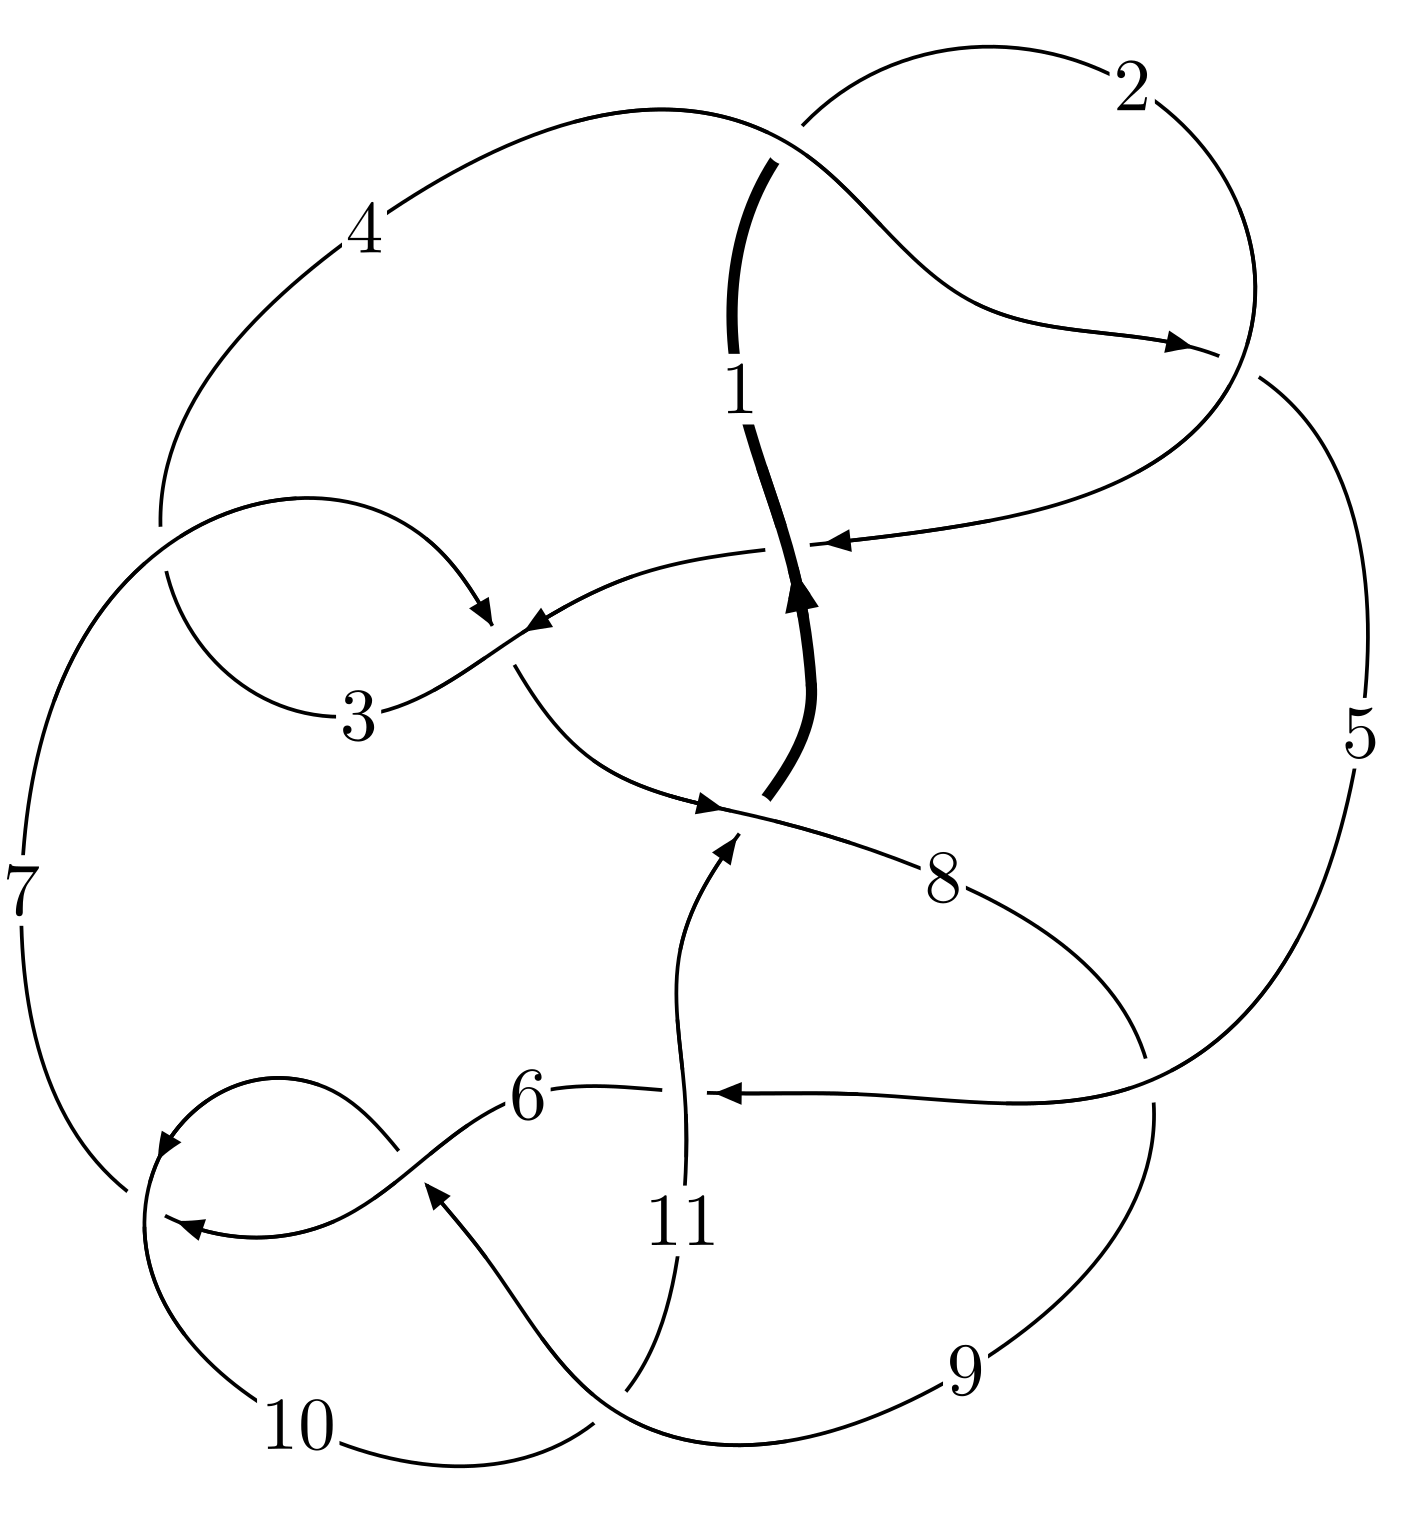
\includegraphics[width=112pt]{../../../GIT/diagram.site/Diagrams/png/281_11a_32.png}\\
\ \ \ A knot diagram\footnotemark}&
\allowdisplaybreaks
\textbf{Linearized knot diagam} \\
\cline{2-2}
 &
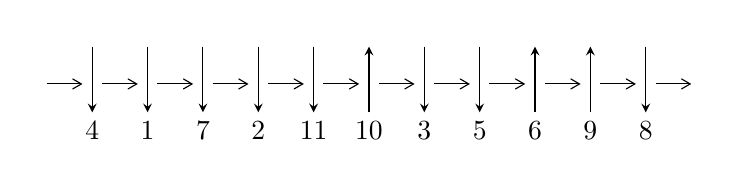
\begin{tikzpicture}[x=20pt, y=17pt]
	% nodes
	\node (C0) at (0, 0) {};
	\node (C1) at (1, 0) {};
	\node (C1U) at (1, +1) {};
	\node (C1D) at (1, -1) {4};

	\node (C2) at (2, 0) {};
	\node (C2U) at (2, +1) {};
	\node (C2D) at (2, -1) {1};

	\node (C3) at (3, 0) {};
	\node (C3U) at (3, +1) {};
	\node (C3D) at (3, -1) {7};

	\node (C4) at (4, 0) {};
	\node (C4U) at (4, +1) {};
	\node (C4D) at (4, -1) {2};

	\node (C5) at (5, 0) {};
	\node (C5U) at (5, +1) {};
	\node (C5D) at (5, -1) {11};

	\node (C6) at (6, 0) {};
	\node (C6U) at (6, +1) {};
	\node (C6D) at (6, -1) {10};

	\node (C7) at (7, 0) {};
	\node (C7U) at (7, +1) {};
	\node (C7D) at (7, -1) {3};

	\node (C8) at (8, 0) {};
	\node (C8U) at (8, +1) {};
	\node (C8D) at (8, -1) {5};

	\node (C9) at (9, 0) {};
	\node (C9U) at (9, +1) {};
	\node (C9D) at (9, -1) {6};

	\node (C10) at (10, 0) {};
	\node (C10U) at (10, +1) {};
	\node (C10D) at (10, -1) {9};

	\node (C11) at (11, 0) {};
	\node (C11U) at (11, +1) {};
	\node (C11D) at (11, -1) {8};
	\node (C12) at (12, 0) {};

	% arrows
	\draw[->,>={angle 60}]
	(C0) edge (C1) (C1) edge (C2) (C2) edge (C3) (C3) edge (C4) (C4) edge (C5) (C5) edge (C6) (C6) edge (C7) (C7) edge (C8) (C8) edge (C9) (C9) edge (C10) (C10) edge (C11) (C11) edge (C12) ;	\draw[->,>=stealth]
	(C1U) edge (C1D) (C2U) edge (C2D) (C3U) edge (C3D) (C4U) edge (C4D) (C5U) edge (C5D) (C6D) edge (C6U) (C7U) edge (C7D) (C8U) edge (C8D) (C9D) edge (C9U) (C10D) edge (C10U) (C11U) edge (C11D) ;
	\end{tikzpicture} \\
\hhline{~~} \\& 
\textbf{Solving Sequence} \\ \cline{2-2} 
 &
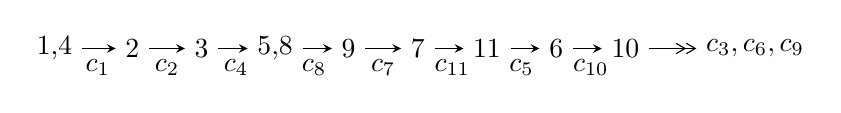
\begin{tikzpicture}[x=25pt, y=7pt]
	% node
	\node (A0) at (-1/8, 0) {1,4};
	\node (A1) at (1, 0) {2};
	\node (A2) at (2, 0) {3};
	\node (A3) at (49/16, 0) {5,8};
	\node (A4) at (33/8, 0) {9};
	\node (A5) at (41/8, 0) {7};
	\node (A6) at (49/8, 0) {11};
	\node (A7) at (57/8, 0) {6};
	\node (A8) at (65/8, 0) {10};
	\node (C1) at (1/2, -1) {$c_{1}$};
	\node (C2) at (3/2, -1) {$c_{2}$};
	\node (C3) at (5/2, -1) {$c_{4}$};
	\node (C4) at (29/8, -1) {$c_{8}$};
	\node (C5) at (37/8, -1) {$c_{7}$};
	\node (C6) at (45/8, -1) {$c_{11}$};
	\node (C7) at (53/8, -1) {$c_{5}$};
	\node (C8) at (61/8, -1) {$c_{10}$};
	\node (A9) at (10, 0) {$c_{3},c_{6},c_{9}$};

	% edge
	\draw[->,>=stealth]	
	(A0) edge (A1) (A1) edge (A2) (A2) edge (A3) (A3) edge (A4) (A4) edge (A5) (A5) edge (A6) (A6) edge (A7) (A7) edge (A8) ;
	\draw[->>,>={angle 60}]	
	(A8) edge (A9);
\end{tikzpicture} \\ 

\end{tabular} \\

\footnotetext{
The image of knot diagram is generated by the software ``\textbf{Draw programme}" developed by Andrew Bartholomew(\url{http://www.layer8.co.uk/maths/draw/index.htm\#Running-draw}), where we modified some parts for our purpose(\url{https://github.com/CATsTAILs/LinksPainter}).
}\phantom \\ \newline 
\centering \textbf{Ideals for irreducible components\footnotemark of $X_{\text{par}}$} 
 
\begin{align*}
I^u_{1}&=\langle 
-2667 u^{74}-16330 u^{73}+\cdots+32 b+2491,\;-73 u^{74}-402 u^{73}+\cdots+4 a+14,\\
\phantom{I^u_{1}}&\phantom{= \langle  }u^{75}+7 u^{74}+\cdots-5 u-1\rangle \\
I^u_{2}&=\langle 
b^6- b^5- b^4+2 b^3- b+1,\;a,\;u-1\rangle \\
\\
\end{align*}
\raggedright * 2 irreducible components of $\dim_{\mathbb{C}}=0$, with total 81 representations.\\
\footnotetext{All coefficients of polynomials are rational numbers. But the coefficients are sometimes approximated in decimal forms when there is not enough margin.}
\newpage
\renewcommand{\arraystretch}{1}
\centering \section*{I. $I^u_{1}= \langle -2667 u^{74}-16330 u^{73}+\cdots+32 b+2491,\;-73 u^{74}-402 u^{73}+\cdots+4 a+14,\;u^{75}+7 u^{74}+\cdots-5 u-1 \rangle$}
\flushleft \textbf{(i) Arc colorings}\\
\begin{tabular}{m{7pt} m{180pt} m{7pt} m{180pt} }
\flushright $a_{1}=$&$\begin{pmatrix}1\\0\end{pmatrix}$ \\
\flushright $a_{4}=$&$\begin{pmatrix}0\\u\end{pmatrix}$ \\
\flushright $a_{2}=$&$\begin{pmatrix}1\\u^2\end{pmatrix}$ \\
\flushright $a_{3}=$&$\begin{pmatrix}- u^2+1\\u^2\end{pmatrix}$ \\
\flushright $a_{5}=$&$\begin{pmatrix}- u\\- u^3+u\end{pmatrix}$ \\
\flushright $a_{8}=$&$\begin{pmatrix}\frac{73}{4} u^{74}+\frac{201}{2} u^{73}+\cdots-28 u-\frac{7}{2}\\83.3438 u^{74}+510.313 u^{73}+\cdots-333.875 u-77.8438\end{pmatrix}$ \\
\flushright $a_{9}=$&$\begin{pmatrix}-46.8438 u^{74}-314.063 u^{73}+\cdots+281.125 u+72.8438\\139.344 u^{74}+836.563 u^{73}+\cdots-502.625 u-113.094\end{pmatrix}$ \\
\flushright $a_{7}=$&$\begin{pmatrix}-\frac{45}{2} u^{74}-161 u^{73}+\cdots+171 u+\frac{185}{4}\\127.594 u^{74}+769.063 u^{73}+\cdots-466.625 u-105.094\end{pmatrix}$ \\
\flushright $a_{11}=$&$\begin{pmatrix}- u^7+2 u^5+2 u^4-2 u^3-2 u^2+2\\\frac{1}{32} u^{74}+\frac{3}{16} u^{73}+\cdots-\frac{9}{8} u-\frac{1}{32}\end{pmatrix}$ \\
\flushright $a_{6}=$&$\begin{pmatrix}\frac{3}{32} u^{74}+\frac{9}{16} u^{73}+\cdots-\frac{43}{8} u-\frac{3}{32}\\1.28125 u^{74}+7.75000 u^{73}+\cdots-4.31250 u-1.34375\end{pmatrix}$ \\
\flushright $a_{10}=$&$\begin{pmatrix}1.06250 u^{74}+6.43750 u^{73}+\cdots-2.43750 u-0.125000\\-1.34375 u^{74}-8.12500 u^{73}+\cdots+5.56250 u+1.40625\end{pmatrix}$\\ \flushright $a_{10}=$&$\begin{pmatrix}1.06250 u^{74}+6.43750 u^{73}+\cdots-2.43750 u-0.125000\\-1.34375 u^{74}-8.12500 u^{73}+\cdots+5.56250 u+1.40625\end{pmatrix}$\\&\end{tabular}
\flushleft \textbf{(ii) Obstruction class $= -1$}\\~\\
\flushleft \textbf{(iii) Cusp Shapes $= \frac{1275}{8} u^{74}+\frac{15911}{16} u^{73}+\cdots-\frac{11065}{16} u-\frac{2603}{16}$}\\~\\
\newpage\renewcommand{\arraystretch}{1}
\flushleft \textbf{(iv) u-Polynomials at the component}\newline \\
\begin{tabular}{m{50pt}|m{274pt}}
Crossings & \hspace{64pt}u-Polynomials at each crossing \\
\hline $$\begin{aligned}c_{1},c_{4}\end{aligned}$$&$\begin{aligned}
&u^{75}-7 u^{74}+\cdots-5 u+1
\end{aligned}$\\
\hline $$\begin{aligned}c_{2}\end{aligned}$$&$\begin{aligned}
&u^{75}+35 u^{74}+\cdots+5 u+1
\end{aligned}$\\
\hline $$\begin{aligned}c_{3},c_{7}\end{aligned}$$&$\begin{aligned}
&u^{75}+u^{74}+\cdots+128 u+64
\end{aligned}$\\
\hline $$\begin{aligned}c_{5}\end{aligned}$$&$\begin{aligned}
&u^{75}-6 u^{74}+\cdots-164 u+77
\end{aligned}$\\
\hline $$\begin{aligned}c_{6},c_{9}\end{aligned}$$&$\begin{aligned}
&u^{75}-2 u^{74}+\cdots-6 u^2+1
\end{aligned}$\\
\hline $$\begin{aligned}c_{8}\end{aligned}$$&$\begin{aligned}
&u^{75}+2 u^{74}+\cdots+126 u+9
\end{aligned}$\\
\hline $$\begin{aligned}c_{10}\end{aligned}$$&$\begin{aligned}
&u^{75}-36 u^{74}+\cdots+12 u-1
\end{aligned}$\\
\hline $$\begin{aligned}c_{11}\end{aligned}$$&$\begin{aligned}
&u^{75}-8 u^{74}+\cdots+26798 u-565
\end{aligned}$\\
\hline
\end{tabular}\\~\\
\newpage\renewcommand{\arraystretch}{1}
\flushleft \textbf{(v) Riley Polynomials at the component}\newline \\
\begin{tabular}{m{50pt}|m{274pt}}
Crossings & \hspace{64pt}Riley Polynomials at each crossing \\
\hline $$\begin{aligned}c_{1},c_{4}\end{aligned}$$&$\begin{aligned}
&y^{75}-35 y^{74}+\cdots+5 y-1
\end{aligned}$\\
\hline $$\begin{aligned}c_{2}\end{aligned}$$&$\begin{aligned}
&y^{75}+17 y^{74}+\cdots-207 y-1
\end{aligned}$\\
\hline $$\begin{aligned}c_{3},c_{7}\end{aligned}$$&$\begin{aligned}
&y^{75}+39 y^{74}+\cdots-61440 y-4096
\end{aligned}$\\
\hline $$\begin{aligned}c_{5}\end{aligned}$$&$\begin{aligned}
&y^{75}+20 y^{74}+\cdots-398760 y-5929
\end{aligned}$\\
\hline $$\begin{aligned}c_{6},c_{9}\end{aligned}$$&$\begin{aligned}
&y^{75}-36 y^{74}+\cdots+12 y-1
\end{aligned}$\\
\hline $$\begin{aligned}c_{8}\end{aligned}$$&$\begin{aligned}
&y^{75}-12 y^{74}+\cdots+2088 y-81
\end{aligned}$\\
\hline $$\begin{aligned}c_{10}\end{aligned}$$&$\begin{aligned}
&y^{75}+8 y^{74}+\cdots+56 y-1
\end{aligned}$\\
\hline $$\begin{aligned}c_{11}\end{aligned}$$&$\begin{aligned}
&y^{75}+24 y^{74}+\cdots+571587624 y-319225
\end{aligned}$\\
\hline
\end{tabular}\\~\\
\newpage\flushleft \textbf{(vi) Complex Volumes and Cusp Shapes}
$$\begin{array}{c|c|c}  
\text{Solutions to }I^u_{1}& \I (\text{vol} + \sqrt{-1}CS) & \text{Cusp shape}\\
 \hline 
\begin{aligned}
u &= -0.406046 + 0.914346 I \\
a &= -0.83062 - 1.51440 I \\
b &= \phantom{-}0.60234 + 1.46500 I\end{aligned}
 & \phantom{-}5.40227 - 10.31970 I & \phantom{-0.000000 } 0 \\ \hline\begin{aligned}
u &= -0.406046 - 0.914346 I \\
a &= -0.83062 + 1.51440 I \\
b &= \phantom{-}0.60234 - 1.46500 I\end{aligned}
 & \phantom{-}5.40227 + 10.31970 I & \phantom{-0.000000 } 0 \\ \hline\begin{aligned}
u &= -0.454473 + 0.894363 I \\
a &= -0.56950 - 1.42313 I \\
b &= \phantom{-}0.45430 + 1.38825 I\end{aligned}
 & \phantom{-}7.45504 - 2.41458 I & \phantom{-0.000000 } 0 \\ \hline\begin{aligned}
u &= -0.454473 - 0.894363 I \\
a &= -0.56950 + 1.42313 I \\
b &= \phantom{-}0.45430 - 1.38825 I\end{aligned}
 & \phantom{-}7.45504 + 2.41458 I & \phantom{-0.000000 } 0 \\ \hline\begin{aligned}
u &= -0.616299 + 0.807630 I \\
a &= \phantom{-}0.160572 - 0.892832 I \\
b &= \phantom{-}0.141279 + 0.953665 I\end{aligned}
 & \phantom{-}4.34347 + 1.49968 I & \phantom{-0.000000 } 0 \\ \hline\begin{aligned}
u &= -0.616299 - 0.807630 I \\
a &= \phantom{-}0.160572 + 0.892832 I \\
b &= \phantom{-}0.141279 - 0.953665 I\end{aligned}
 & \phantom{-}4.34347 - 1.49968 I & \phantom{-0.000000 } 0 \\ \hline\begin{aligned}
u &= -0.408706 + 0.889849 I \\
a &= \phantom{-}0.80491 + 1.38796 I \\
b &= -0.59555 - 1.38804 I\end{aligned}
 & \phantom{-}2.98486 - 5.33708 I & \phantom{-0.000000 } 0 \\ \hline\begin{aligned}
u &= -0.408706 - 0.889849 I \\
a &= \phantom{-}0.80491 - 1.38796 I \\
b &= -0.59555 + 1.38804 I\end{aligned}
 & \phantom{-}2.98486 + 5.33708 I & \phantom{-0.000000 } 0 \\ \hline\begin{aligned}
u &= -0.843169 + 0.484968 I \\
a &= \phantom{-}0.203680 + 0.416849 I \\
b &= \phantom{-}0.961078 + 0.362588 I\end{aligned}
 & \phantom{-}1.69304 + 2.02908 I & \phantom{-0.000000 } 0 \\ \hline\begin{aligned}
u &= -0.843169 - 0.484968 I \\
a &= \phantom{-}0.203680 - 0.416849 I \\
b &= \phantom{-}0.961078 - 0.362588 I\end{aligned}
 & \phantom{-}1.69304 - 2.02908 I & \phantom{-0.000000 } 0\\
 \hline 
 \end{array}$$\newpage$$\begin{array}{c|c|c}  
\text{Solutions to }I^u_{1}& \I (\text{vol} + \sqrt{-1}CS) & \text{Cusp shape}\\
 \hline 
\begin{aligned}
u &= -0.891387 + 0.371717 I \\
a &= -0.033242 - 0.565045 I \\
b &= -1.42939 - 0.58093 I\end{aligned}
 & -3.04790 + 0.34112 I & \phantom{-0.000000 } 0 \\ \hline\begin{aligned}
u &= -0.891387 - 0.371717 I \\
a &= -0.033242 + 0.565045 I \\
b &= -1.42939 + 0.58093 I\end{aligned}
 & -3.04790 - 0.34112 I & \phantom{-0.000000 } 0 \\ \hline\begin{aligned}
u &= -0.582384 + 0.856983 I \\
a &= -0.062854 + 1.166120 I \\
b &= -0.127560 - 1.134840 I\end{aligned}
 & \phantom{-}8.27872 - 1.80903 I & \phantom{-0.000000 } 0 \\ \hline\begin{aligned}
u &= -0.582384 - 0.856983 I \\
a &= -0.062854 - 1.166120 I \\
b &= -0.127560 + 1.134840 I\end{aligned}
 & \phantom{-}8.27872 + 1.80903 I & \phantom{-0.000000 } 0 \\ \hline\begin{aligned}
u &= -0.959321 + 0.422476 I \\
a &= -0.127985 - 0.694740 I \\
b &= -1.52139 - 0.15181 I\end{aligned}
 & -3.43299 + 2.76594 I & \phantom{-0.000000 } 0 \\ \hline\begin{aligned}
u &= -0.959321 - 0.422476 I \\
a &= -0.127985 + 0.694740 I \\
b &= -1.52139 + 0.15181 I\end{aligned}
 & -3.43299 - 2.76594 I & \phantom{-0.000000 } 0 \\ \hline\begin{aligned}
u &= -0.648496 + 0.836558 I \\
a &= -0.351520 + 0.975110 I \\
b &= -0.006205 - 0.945446 I\end{aligned}
 & \phantom{-}6.99192 + 6.13645 I & \phantom{-0.000000 } 0 \\ \hline\begin{aligned}
u &= -0.648496 - 0.836558 I \\
a &= -0.351520 - 0.975110 I \\
b &= -0.006205 + 0.945446 I\end{aligned}
 & \phantom{-}6.99192 - 6.13645 I & \phantom{-0.000000 } 0 \\ \hline\begin{aligned}
u &= -0.868237 + 0.338548 I \\
a &= -0.012725 + 0.536185 I \\
b &= \phantom{-}1.41093 + 0.77808 I\end{aligned}
 & -1.13942 - 4.67222 I & \phantom{-0.000000 } 0 \\ \hline\begin{aligned}
u &= -0.868237 - 0.338548 I \\
a &= -0.012725 - 0.536185 I \\
b &= \phantom{-}1.41093 - 0.77808 I\end{aligned}
 & -1.13942 + 4.67222 I & \phantom{-0.000000 } 0\\
 \hline 
 \end{array}$$\newpage$$\begin{array}{c|c|c}  
\text{Solutions to }I^u_{1}& \I (\text{vol} + \sqrt{-1}CS) & \text{Cusp shape}\\
 \hline 
\begin{aligned}
u &= \phantom{-}0.921822 + 0.543679 I \\
a &= \phantom{-}0.80291 - 1.93730 I \\
b &= \phantom{-}0.450724 + 1.151160 I\end{aligned}
 & \phantom{-}2.49508 - 2.11040 I & \phantom{-0.000000 } 0 \\ \hline\begin{aligned}
u &= \phantom{-}0.921822 - 0.543679 I \\
a &= \phantom{-}0.80291 + 1.93730 I \\
b &= \phantom{-}0.450724 - 1.151160 I\end{aligned}
 & \phantom{-}2.49508 + 2.11040 I & \phantom{-0.000000 } 0 \\ \hline\begin{aligned}
u &= \phantom{-}0.744498 + 0.529322 I \\
a &= -1.44577 + 1.56624 I \\
b &= \phantom{-}0.149282 - 0.958064 I\end{aligned}
 & \phantom{-}3.05917 - 2.25044 I & \phantom{-0.000000 } 0 \\ \hline\begin{aligned}
u &= \phantom{-}0.744498 - 0.529322 I \\
a &= -1.44577 - 1.56624 I \\
b &= \phantom{-}0.149282 + 0.958064 I\end{aligned}
 & \phantom{-}3.05917 + 2.25044 I & \phantom{-0.000000 } 0 \\ \hline\begin{aligned}
u &= -0.993853 + 0.440511 I \\
a &= \phantom{-}0.166101 + 0.783333 I \\
b &= \phantom{-}1.56989 - 0.06150 I\end{aligned}
 & -1.89293 + 7.72902 I & \phantom{-0.000000 } 0 \\ \hline\begin{aligned}
u &= -0.993853 - 0.440511 I \\
a &= \phantom{-}0.166101 - 0.783333 I \\
b &= \phantom{-}1.56989 + 0.06150 I\end{aligned}
 & -1.89293 - 7.72902 I & \phantom{-0.000000 } 0 \\ \hline\begin{aligned}
u &= \phantom{-}1.004560 + 0.452388 I \\
a &= -0.33920 + 1.62466 I \\
b &= -0.761658 - 0.767228 I\end{aligned}
 & -3.12121 - 3.06401 I & \phantom{-0.000000 } 0 \\ \hline\begin{aligned}
u &= \phantom{-}1.004560 - 0.452388 I \\
a &= -0.33920 - 1.62466 I \\
b &= -0.761658 + 0.767228 I\end{aligned}
 & -3.12121 + 3.06401 I & \phantom{-0.000000 } 0 \\ \hline\begin{aligned}
u &= -0.395112 + 0.797470 I \\
a &= \phantom{-}0.829656 + 0.944652 I \\
b &= -0.635642 - 1.147260 I\end{aligned}
 & \phantom{-}1.26952 - 3.45416 I & \phantom{-0.000000 } 0 \\ \hline\begin{aligned}
u &= -0.395112 - 0.797470 I \\
a &= \phantom{-}0.829656 - 0.944652 I \\
b &= -0.635642 + 1.147260 I\end{aligned}
 & \phantom{-}1.26952 + 3.45416 I & \phantom{-0.000000 } 0\\
 \hline 
 \end{array}$$\newpage$$\begin{array}{c|c|c}  
\text{Solutions to }I^u_{1}& \I (\text{vol} + \sqrt{-1}CS) & \text{Cusp shape}\\
 \hline 
\begin{aligned}
u &= \phantom{-}0.976476 + 0.533746 I \\
a &= -0.54173 + 1.96861 I \\
b &= -0.682122 - 1.116880 I\end{aligned}
 & -1.82400 - 4.84040 I & \phantom{-0.000000 } 0 \\ \hline\begin{aligned}
u &= \phantom{-}0.976476 - 0.533746 I \\
a &= -0.54173 - 1.96861 I \\
b &= -0.682122 + 1.116880 I\end{aligned}
 & -1.82400 + 4.84040 I & \phantom{-0.000000 } 0 \\ \hline\begin{aligned}
u &= \phantom{-}1.046730 + 0.394188 I \\
a &= \phantom{-}0.135208 - 1.388780 I \\
b &= \phantom{-}0.855036 + 0.498982 I\end{aligned}
 & -2.04922 + 1.40109 I & \phantom{-0.000000 } 0 \\ \hline\begin{aligned}
u &= \phantom{-}1.046730 - 0.394188 I \\
a &= \phantom{-}0.135208 + 1.388780 I \\
b &= \phantom{-}0.855036 - 0.498982 I\end{aligned}
 & -2.04922 - 1.40109 I & \phantom{-0.000000 } 0 \\ \hline\begin{aligned}
u &= \phantom{-}0.980018 + 0.559884 I \\
a &= \phantom{-}0.55911 - 2.09753 I \\
b &= \phantom{-}0.69820 + 1.23354 I\end{aligned}
 & \phantom{-}0.49666 - 9.74933 I & \phantom{-0.000000 } 0 \\ \hline\begin{aligned}
u &= \phantom{-}0.980018 - 0.559884 I \\
a &= \phantom{-}0.55911 + 2.09753 I \\
b &= \phantom{-}0.69820 - 1.23354 I\end{aligned}
 & \phantom{-}0.49666 + 9.74933 I & \phantom{-0.000000 } 0 \\ \hline\begin{aligned}
u &= \phantom{-}0.625774 + 0.553199 I \\
a &= -1.82685 + 1.38552 I \\
b &= \phantom{-}0.488149 - 0.843348 I\end{aligned}
 & \phantom{-}1.56352 + 5.23293 I & \phantom{-0.000000 } 0 \\ \hline\begin{aligned}
u &= \phantom{-}0.625774 - 0.553199 I \\
a &= -1.82685 - 1.38552 I \\
b &= \phantom{-}0.488149 + 0.843348 I\end{aligned}
 & \phantom{-}1.56352 - 5.23293 I & \phantom{-0.000000 } 0 \\ \hline\begin{aligned}
u &= -0.428137 + 0.690269 I \\
a &= -0.668511 - 0.521270 I \\
b &= \phantom{-}0.588098 + 0.950437 I\end{aligned}
 & \phantom{-}1.89347 + 1.09587 I & -2.44221 - 2.55300 I \\ \hline\begin{aligned}
u &= -0.428137 - 0.690269 I \\
a &= -0.668511 + 0.521270 I \\
b &= \phantom{-}0.588098 - 0.950437 I\end{aligned}
 & \phantom{-}1.89347 - 1.09587 I & -2.44221 + 2.55300 I\\
 \hline 
 \end{array}$$\newpage$$\begin{array}{c|c|c}  
\text{Solutions to }I^u_{1}& \I (\text{vol} + \sqrt{-1}CS) & \text{Cusp shape}\\
 \hline 
\begin{aligned}
u &= \phantom{-}1.170610 + 0.255451 I \\
a &= -0.271560 - 0.787523 I \\
b &= \phantom{-}0.928676 - 0.247240 I\end{aligned}
 & -2.42380 - 3.72637 I & \phantom{-0.000000 } 0 \\ \hline\begin{aligned}
u &= \phantom{-}1.170610 - 0.255451 I \\
a &= -0.271560 + 0.787523 I \\
b &= \phantom{-}0.928676 + 0.247240 I\end{aligned}
 & -2.42380 + 3.72637 I & \phantom{-0.000000 } 0 \\ \hline\begin{aligned}
u &= \phantom{-}1.195250 + 0.198323 I \\
a &= \phantom{-}0.271492 + 0.579940 I \\
b &= -0.788651 + 0.477728 I\end{aligned}
 & -3.76765 + 0.74515 I & \phantom{-0.000000 } 0 \\ \hline\begin{aligned}
u &= \phantom{-}1.195250 - 0.198323 I \\
a &= \phantom{-}0.271492 - 0.579940 I \\
b &= -0.788651 - 0.477728 I\end{aligned}
 & -3.76765 - 0.74515 I & \phantom{-0.000000 } 0 \\ \hline\begin{aligned}
u &= -1.014220 + 0.671104 I \\
a &= \phantom{-}1.008370 + 0.729025 I \\
b &= \phantom{-}0.428776 - 0.699364 I\end{aligned}
 & \phantom{-}3.13966 + 4.03622 I & \phantom{-0.000000 } 0 \\ \hline\begin{aligned}
u &= -1.014220 - 0.671104 I \\
a &= \phantom{-}1.008370 - 0.729025 I \\
b &= \phantom{-}0.428776 + 0.699364 I\end{aligned}
 & \phantom{-}3.13966 - 4.03622 I & \phantom{-0.000000 } 0 \\ \hline\begin{aligned}
u &= \phantom{-}0.625476 + 0.471165 I \\
a &= \phantom{-}1.67010 - 1.18891 I \\
b &= -0.365304 + 0.668182 I\end{aligned}
 & -0.750144 + 0.597052 I & -5.79846 + 0. I\phantom{ +0.000000I} \\ \hline\begin{aligned}
u &= \phantom{-}0.625476 - 0.471165 I \\
a &= \phantom{-}1.67010 + 1.18891 I \\
b &= -0.365304 - 0.668182 I\end{aligned}
 & -0.750144 - 0.597052 I & -5.79846 + 0. I\phantom{ +0.000000I} \\ \hline\begin{aligned}
u &= -0.996956 + 0.705289 I \\
a &= -1.135140 - 0.591809 I \\
b &= -0.214156 + 0.626907 I\end{aligned}
 & \phantom{-}5.93451 - 0.41079 I & \phantom{-0.000000 } 0 \\ \hline\begin{aligned}
u &= -0.996956 - 0.705289 I \\
a &= -1.135140 + 0.591809 I \\
b &= -0.214156 - 0.626907 I\end{aligned}
 & \phantom{-}5.93451 + 0.41079 I & \phantom{-0.000000 } 0\\
 \hline 
 \end{array}$$\newpage$$\begin{array}{c|c|c}  
\text{Solutions to }I^u_{1}& \I (\text{vol} + \sqrt{-1}CS) & \text{Cusp shape}\\
 \hline 
\begin{aligned}
u &= \phantom{-}0.777815\phantom{ +0.000000I} \\
a &= \phantom{-}0.931575\phantom{ +0.000000I} \\
b &= \phantom{-}0.0235617\phantom{ +0.000000I}\end{aligned}
 & -1.12557\phantom{ +0.000000I} & -9.38810\phantom{ +0.000000I} \\ \hline\begin{aligned}
u &= -1.096560 + 0.590139 I \\
a &= \phantom{-}0.699149 + 1.173110 I \\
b &= \phantom{-}1.06597 - 1.05792 I\end{aligned}
 & -0.07882 + 3.89973 I & \phantom{-0.000000 } 0 \\ \hline\begin{aligned}
u &= -1.096560 - 0.590139 I \\
a &= \phantom{-}0.699149 - 1.173110 I \\
b &= \phantom{-}1.06597 + 1.05792 I\end{aligned}
 & -0.07882 - 3.89973 I & \phantom{-0.000000 } 0 \\ \hline\begin{aligned}
u &= -1.050220 + 0.693988 I \\
a &= -1.17073 - 0.86818 I \\
b &= -0.326464 + 0.944045 I\end{aligned}
 & \phantom{-}6.86340 + 7.55493 I & \phantom{-0.000000 } 0 \\ \hline\begin{aligned}
u &= -1.050220 - 0.693988 I \\
a &= -1.17073 + 0.86818 I \\
b &= -0.326464 - 0.944045 I\end{aligned}
 & \phantom{-}6.86340 - 7.55493 I & \phantom{-0.000000 } 0 \\ \hline\begin{aligned}
u &= \phantom{-}1.267990 + 0.074126 I \\
a &= -0.176506 - 0.199334 I \\
b &= \phantom{-}0.364909 - 0.990702 I\end{aligned}
 & \phantom{-}1.311430 - 0.241237 I & \phantom{-0.000000 } 0 \\ \hline\begin{aligned}
u &= \phantom{-}1.267990 - 0.074126 I \\
a &= -0.176506 + 0.199334 I \\
b &= \phantom{-}0.364909 + 0.990702 I\end{aligned}
 & \phantom{-}1.311430 + 0.241237 I & \phantom{-0.000000 } 0 \\ \hline\begin{aligned}
u &= \phantom{-}1.263610 + 0.138529 I \\
a &= \phantom{-}0.321540 + 0.309132 I \\
b &= -0.669397 + 0.885758 I\end{aligned}
 & -2.79598 + 2.38150 I & \phantom{-0.000000 } 0 \\ \hline\begin{aligned}
u &= \phantom{-}1.263610 - 0.138529 I \\
a &= \phantom{-}0.321540 - 0.309132 I \\
b &= -0.669397 - 0.885758 I\end{aligned}
 & -2.79598 - 2.38150 I & \phantom{-0.000000 } 0 \\ \hline\begin{aligned}
u &= -1.120130 + 0.610216 I \\
a &= -0.79865 - 1.28631 I \\
b &= -0.99237 + 1.25830 I\end{aligned}
 & -0.87148 + 8.74235 I & \phantom{-0.000000 } 0\\
 \hline 
 \end{array}$$\newpage$$\begin{array}{c|c|c}  
\text{Solutions to }I^u_{1}& \I (\text{vol} + \sqrt{-1}CS) & \text{Cusp shape}\\
 \hline 
\begin{aligned}
u &= -1.120130 - 0.610216 I \\
a &= -0.79865 + 1.28631 I \\
b &= -0.99237 - 1.25830 I\end{aligned}
 & -0.87148 - 8.74235 I & \phantom{-0.000000 } 0 \\ \hline\begin{aligned}
u &= \phantom{-}1.292750 + 0.134584 I \\
a &= -0.368918 - 0.227788 I \\
b &= \phantom{-}0.699572 - 1.035680 I\end{aligned}
 & -0.53723 + 7.20125 I & \phantom{-0.000000 } 0 \\ \hline\begin{aligned}
u &= \phantom{-}1.292750 - 0.134584 I \\
a &= -0.368918 + 0.227788 I \\
b &= \phantom{-}0.699572 + 1.035680 I\end{aligned}
 & -0.53723 - 7.20125 I & \phantom{-0.000000 } 0 \\ \hline\begin{aligned}
u &= -1.129100 + 0.660193 I \\
a &= \phantom{-}1.06700 + 1.32077 I \\
b &= \phantom{-}0.66904 - 1.42604 I\end{aligned}
 & \phantom{-}5.41191 + 8.13992 I & \phantom{-0.000000 } 0 \\ \hline\begin{aligned}
u &= -1.129100 - 0.660193 I \\
a &= \phantom{-}1.06700 - 1.32077 I \\
b &= \phantom{-}0.66904 + 1.42604 I\end{aligned}
 & \phantom{-}5.41191 - 8.13992 I & \phantom{-0.000000 } 0 \\ \hline\begin{aligned}
u &= -1.145670 + 0.642227 I \\
a &= -0.97178 - 1.41886 I \\
b &= -0.83020 + 1.50674 I\end{aligned}
 & \phantom{-}0.76093 + 10.98050 I & \phantom{-0.000000 } 0 \\ \hline\begin{aligned}
u &= -1.145670 - 0.642227 I \\
a &= -0.97178 + 1.41886 I \\
b &= -0.83020 - 1.50674 I\end{aligned}
 & \phantom{-}0.76093 - 10.98050 I & \phantom{-0.000000 } 0 \\ \hline\begin{aligned}
u &= -1.155510 + 0.649574 I \\
a &= \phantom{-}1.01483 + 1.47364 I \\
b &= \phantom{-}0.79889 - 1.59357 I\end{aligned}
 & \phantom{-}3.1307 + 16.0547 I & \phantom{-0.000000 } 0 \\ \hline\begin{aligned}
u &= -1.155510 - 0.649574 I \\
a &= \phantom{-}1.01483 - 1.47364 I \\
b &= \phantom{-}0.79889 + 1.59357 I\end{aligned}
 & \phantom{-}3.1307 - 16.0547 I & \phantom{-0.000000 } 0 \\ \hline\begin{aligned}
u &= \phantom{-}0.147490 + 0.463827 I \\
a &= -2.03597 + 0.59027 I \\
b &= \phantom{-}0.787606 + 0.109338 I\end{aligned}
 & \phantom{-}0.40746 - 4.84347 I & -2.88894 + 6.95560 I\\
 \hline 
 \end{array}$$\newpage$$\begin{array}{c|c|c}  
\text{Solutions to }I^u_{1}& \I (\text{vol} + \sqrt{-1}CS) & \text{Cusp shape}\\
 \hline 
\begin{aligned}
u &= \phantom{-}0.147490 - 0.463827 I \\
a &= -2.03597 - 0.59027 I \\
b &= \phantom{-}0.787606 - 0.109338 I\end{aligned}
 & \phantom{-}0.40746 + 4.84347 I & -2.88894 - 6.95560 I \\ \hline\begin{aligned}
u &= \phantom{-}0.267477 + 0.336990 I \\
a &= \phantom{-}2.04829 - 0.66333 I \\
b &= -0.581312 + 0.049909 I\end{aligned}
 & -1.335430 - 0.455559 I & -7.14666 + 1.75479 I \\ \hline\begin{aligned}
u &= \phantom{-}0.267477 - 0.336990 I \\
a &= \phantom{-}2.04829 + 0.66333 I \\
b &= -0.581312 - 0.049909 I\end{aligned}
 & -1.335430 + 0.455559 I & -7.14666 - 1.75479 I \\ \hline\begin{aligned}
u &= -0.215453 + 0.258244 I \\
a &= -0.988925 + 0.959286 I \\
b &= \phantom{-}0.402835 + 0.578892 I\end{aligned}
 & \phantom{-}1.62489 + 1.27832 I & \phantom{-}1.31582 - 1.24706 I \\ \hline\begin{aligned}
u &= -0.215453 - 0.258244 I \\
a &= -0.988925 - 0.959286 I \\
b &= \phantom{-}0.402835 - 0.578892 I\end{aligned}
 & \phantom{-}1.62489 - 1.27832 I & \phantom{-}1.31582 + 1.24706 I\\
 \hline 
 \end{array}$$\newpage\newpage\renewcommand{\arraystretch}{1}
\centering \section*{II. $I^u_{2}= \langle b^6- b^5- b^4+2 b^3- b+1,\;a,\;u-1 \rangle$}
\flushleft \textbf{(i) Arc colorings}\\
\begin{tabular}{m{7pt} m{180pt} m{7pt} m{180pt} }
\flushright $a_{1}=$&$\begin{pmatrix}1\\0\end{pmatrix}$ \\
\flushright $a_{4}=$&$\begin{pmatrix}0\\1\end{pmatrix}$ \\
\flushright $a_{2}=$&$\begin{pmatrix}1\\1\end{pmatrix}$ \\
\flushright $a_{3}=$&$\begin{pmatrix}0\\1\end{pmatrix}$ \\
\flushright $a_{5}=$&$\begin{pmatrix}-1\\0\end{pmatrix}$ \\
\flushright $a_{8}=$&$\begin{pmatrix}0\\b\end{pmatrix}$ \\
\flushright $a_{9}=$&$\begin{pmatrix}- b\\b\end{pmatrix}$ \\
\flushright $a_{7}=$&$\begin{pmatrix}0\\b\end{pmatrix}$ \\
\flushright $a_{11}=$&$\begin{pmatrix}1\\- b^2\end{pmatrix}$ \\
\flushright $a_{6}=$&$\begin{pmatrix}b^2-1\\- b^4\end{pmatrix}$ \\
\flushright $a_{10}=$&$\begin{pmatrix}b^4- b^2+1\\- b^4\end{pmatrix}$\\ \flushright $a_{10}=$&$\begin{pmatrix}b^4- b^2+1\\- b^4\end{pmatrix}$\\&\end{tabular}
\flushleft \textbf{(ii) Obstruction class $= 1$}\\~\\
\flushleft \textbf{(iii) Cusp Shapes $= - b^5+4 b^4+2 b^3-4 b^2+2 b-5$}\\~\\
\newpage\renewcommand{\arraystretch}{1}
\flushleft \textbf{(iv) u-Polynomials at the component}\newline \\
\begin{tabular}{m{50pt}|m{274pt}}
Crossings & \hspace{64pt}u-Polynomials at each crossing \\
\hline $$\begin{aligned}c_{1}\end{aligned}$$&$\begin{aligned}
&(u-1)^6
\end{aligned}$\\
\hline $$\begin{aligned}c_{2},c_{4}\end{aligned}$$&$\begin{aligned}
&(u+1)^6
\end{aligned}$\\
\hline $$\begin{aligned}c_{3},c_{7}\end{aligned}$$&$\begin{aligned}
&u^6
\end{aligned}$\\
\hline $$\begin{aligned}c_{5},c_{10}\end{aligned}$$&$\begin{aligned}
&u^6-3 u^5+5 u^4-4 u^3+2 u^2- u+1
\end{aligned}$\\
\hline $$\begin{aligned}c_{6},c_{8},c_{11}\end{aligned}$$&$\begin{aligned}
&u^6- u^5- u^4+2 u^3- u+1
\end{aligned}$\\
\hline $$\begin{aligned}c_{9}\end{aligned}$$&$\begin{aligned}
&u^6+u^5- u^4-2 u^3+u+1
\end{aligned}$\\
\hline
\end{tabular}\\~\\
\newpage\renewcommand{\arraystretch}{1}
\flushleft \textbf{(v) Riley Polynomials at the component}\newline \\
\begin{tabular}{m{50pt}|m{274pt}}
Crossings & \hspace{64pt}Riley Polynomials at each crossing \\
\hline $$\begin{aligned}c_{1},c_{2},c_{4}\end{aligned}$$&$\begin{aligned}
&(y-1)^6
\end{aligned}$\\
\hline $$\begin{aligned}c_{3},c_{7}\end{aligned}$$&$\begin{aligned}
&y^6
\end{aligned}$\\
\hline $$\begin{aligned}c_{5},c_{10}\end{aligned}$$&$\begin{aligned}
&y^6+y^5+5 y^4+6 y^2+3 y+1
\end{aligned}$\\
\hline $$\begin{aligned}c_{6},c_{8},c_{9}\\c_{11}\end{aligned}$$&$\begin{aligned}
&y^6-3 y^5+5 y^4-4 y^3+2 y^2- y+1
\end{aligned}$\\
\hline
\end{tabular}\\~\\
\newpage\flushleft \textbf{(vi) Complex Volumes and Cusp Shapes}
$$\begin{array}{c|c|c}  
\text{Solutions to }I^u_{2}& \I (\text{vol} + \sqrt{-1}CS) & \text{Cusp shape}\\
 \hline 
\begin{aligned}
u &= \phantom{-}1.00000\phantom{ +0.000000I} \\
a &= \phantom{-0.000000 } 0 \\
b &= -1.002190 + 0.295542 I\end{aligned}
 & -3.53554 + 0.92430 I & -10.03026 - 0.88960 I \\ \hline\begin{aligned}
u &= \phantom{-}1.00000\phantom{ +0.000000I} \\
a &= \phantom{-0.000000 } 0 \\
b &= -1.002190 - 0.295542 I\end{aligned}
 & -3.53554 - 0.92430 I & -10.03026 + 0.88960 I \\ \hline\begin{aligned}
u &= \phantom{-}1.00000\phantom{ +0.000000I} \\
a &= \phantom{-0.000000 } 0 \\
b &= \phantom{-}0.428243 + 0.664531 I\end{aligned}
 & \phantom{-}0.245672 + 0.924305 I & -5.20252 - 1.68215 I \\ \hline\begin{aligned}
u &= \phantom{-}1.00000\phantom{ +0.000000I} \\
a &= \phantom{-0.000000 } 0 \\
b &= \phantom{-}0.428243 - 0.664531 I\end{aligned}
 & \phantom{-}0.245672 - 0.924305 I & -5.20252 + 1.68215 I \\ \hline\begin{aligned}
u &= \phantom{-}1.00000\phantom{ +0.000000I} \\
a &= \phantom{-0.000000 } 0 \\
b &= \phantom{-}1.073950 + 0.558752 I\end{aligned}
 & -1.64493 - 5.69302 I & -6.76721 + 6.15196 I \\ \hline\begin{aligned}
u &= \phantom{-}1.00000\phantom{ +0.000000I} \\
a &= \phantom{-0.000000 } 0 \\
b &= \phantom{-}1.073950 - 0.558752 I\end{aligned}
 & -1.64493 + 5.69302 I & -6.76721 - 6.15196 I\\
 \hline 
 \end{array}$$\newpage
\newpage\renewcommand{\arraystretch}{1}
\centering \section*{ III. u-Polynomials}
\begin{tabular}{m{50pt}|m{274pt}}
Crossings & \hspace{64pt}u-Polynomials at each crossing \\
\hline $$\begin{aligned}c_{1}\end{aligned}$$&$\begin{aligned}
&((u-1)^6)(u^{75}-7 u^{74}+\cdots-5 u+1)
\end{aligned}$\\
\hline $$\begin{aligned}c_{2}\end{aligned}$$&$\begin{aligned}
&((u+1)^6)(u^{75}+35 u^{74}+\cdots+5 u+1)
\end{aligned}$\\
\hline $$\begin{aligned}c_{3},c_{7}\end{aligned}$$&$\begin{aligned}
&u^6(u^{75}+u^{74}+\cdots+128 u+64)
\end{aligned}$\\
\hline $$\begin{aligned}c_{4}\end{aligned}$$&$\begin{aligned}
&((u+1)^6)(u^{75}-7 u^{74}+\cdots-5 u+1)
\end{aligned}$\\
\hline $$\begin{aligned}c_{5}\end{aligned}$$&$\begin{aligned}
&(u^6-3 u^5+5 u^4-4 u^3+2 u^2- u+1)(u^{75}-6 u^{74}+\cdots-164 u+77)
\end{aligned}$\\
\hline $$\begin{aligned}c_{6}\end{aligned}$$&$\begin{aligned}
&(u^6- u^5- u^4+2 u^3- u+1)(u^{75}-2 u^{74}+\cdots-6 u^2+1)
\end{aligned}$\\
\hline $$\begin{aligned}c_{8}\end{aligned}$$&$\begin{aligned}
&(u^6- u^5- u^4+2 u^3- u+1)(u^{75}+2 u^{74}+\cdots+126 u+9)
\end{aligned}$\\
\hline $$\begin{aligned}c_{9}\end{aligned}$$&$\begin{aligned}
&(u^6+u^5- u^4-2 u^3+u+1)(u^{75}-2 u^{74}+\cdots-6 u^2+1)
\end{aligned}$\\
\hline $$\begin{aligned}c_{10}\end{aligned}$$&$\begin{aligned}
&(u^6-3 u^5+5 u^4-4 u^3+2 u^2- u+1)(u^{75}-36 u^{74}+\cdots+12 u-1)
\end{aligned}$\\
\hline $$\begin{aligned}c_{11}\end{aligned}$$&$\begin{aligned}
&(u^6- u^5- u^4+2 u^3- u+1)(u^{75}-8 u^{74}+\cdots+26798 u-565)
\end{aligned}$\\
\hline
\end{tabular}\newpage\renewcommand{\arraystretch}{1}
\centering \section*{ IV. Riley Polynomials}
\begin{tabular}{m{50pt}|m{274pt}}
Crossings & \hspace{64pt}Riley Polynomials at each crossing \\
\hline $$\begin{aligned}c_{1},c_{4}\end{aligned}$$&$\begin{aligned}
&((y-1)^6)(y^{75}-35 y^{74}+\cdots+5 y-1)
\end{aligned}$\\
\hline $$\begin{aligned}c_{2}\end{aligned}$$&$\begin{aligned}
&((y-1)^6)(y^{75}+17 y^{74}+\cdots-207 y-1)
\end{aligned}$\\
\hline $$\begin{aligned}c_{3},c_{7}\end{aligned}$$&$\begin{aligned}
&y^6(y^{75}+39 y^{74}+\cdots-61440 y-4096)
\end{aligned}$\\
\hline $$\begin{aligned}c_{5}\end{aligned}$$&$\begin{aligned}
&(y^6+y^5+5 y^4+6 y^2+3 y+1)(y^{75}+20 y^{74}+\cdots-398760 y-5929)
\end{aligned}$\\
\hline $$\begin{aligned}c_{6},c_{9}\end{aligned}$$&$\begin{aligned}
&(y^6-3 y^5+5 y^4-4 y^3+2 y^2- y+1)(y^{75}-36 y^{74}+\cdots+12 y-1)
\end{aligned}$\\
\hline $$\begin{aligned}c_{8}\end{aligned}$$&$\begin{aligned}
&(y^6-3 y^5+5 y^4-4 y^3+2 y^2- y+1)(y^{75}-12 y^{74}+\cdots+2088 y-81)
\end{aligned}$\\
\hline $$\begin{aligned}c_{10}\end{aligned}$$&$\begin{aligned}
&(y^6+y^5+5 y^4+6 y^2+3 y+1)(y^{75}+8 y^{74}+\cdots+56 y-1)
\end{aligned}$\\
\hline $$\begin{aligned}c_{11}\end{aligned}$$&$\begin{aligned}
&(y^6-3 y^5+5 y^4-4 y^3+2 y^2- y+1)\\
&\cdot(y^{75}+24 y^{74}+\cdots+571587624 y-319225)
\end{aligned}$\\
\hline
\end{tabular}
\vskip 2pc
\end{document}